% Introduction
%
%	Motivation
%	State of the Research
%	Goals and Outline

\chapter{Introduction}

\section{State of knowledge}

In a particle accelerator, the charged particles circulate around the ring and oscillate due to the magnets and the accelerating structures. The accelerating structures, in the \gls{LHC} supra-conducting \glspl{cavity} apply a strong electrical field that oscillates at the \gls{rffreq} to particles in order to collect and accelerate particles in \glspl{bunch} inside a frequency \gls{bucket}.

The particles inside a bucket are oscillating longitudinally along the ring and transversally in the vertical and horizontal plane. The longitudinal oscillations are damped by the beam control system. But the transversal oscillations must be damped by a separate system~: the \gls{ADT}\cite{Benews11,Zhabitsky:1141925}.

One of the key parameters of the accelerator is the betatron tune. The betatron tune, $Q$, is the quotient of the betatron oscillation and the particle frequencies.

$$f_\beta = Q * f_0$$

This value allow us to check if the particle beam is stable and don't reach any dangerous instabilities.

% Literacy survey
\section{Tune measurement in the LHC}

In order to measure the betatron tune in an accelerator we use \glspl{BPM}. These monitors are able to measure the position of the beam in the vacuum chamber.

In the present setup \gls{BI} group is using their \gls{BBQ} \cite{Boccardi:1156349} system to acquire the tune over a certain number of machine turn (256 to 128'000). This can work as a passive instrument or as an on demand system by exciting 12 \glspl{bunch} in the beam with the \gls{MKQA}. \Gls{ADT} has also been used for tune measurement excitation\cite{HofleEvian10}. 

In normal operation, as the \gls{ADT} is active, it is difficult to have a good picture of the excited bunches and make a fine tune measurement~: the oscillations created by the \gls{MKQA} are damped by the \gls{ADT}. There have been studies to disable the \gls{ADT} for a certain number of bunches in order to get a better tune measurement\cite{HofleEvian11}, but this may not be sufficient.

% The source of Ideas
\section{Proposed system}

The \gls{ADT} also have \glspl{BPM} and these can have per bunch measurement\cite{BphMeas07}. This could allow a much precise measurement. But due to the high among of data to be processed (estimated to 640 mega bytes per seconds for each \gls{BPM}) dedicated hardware is needed to compute the correct tune\cite{HofleChamonix12}.

In order to be able to apply direct correction to beam oscilliation the \gls{tune} has to be measured at a high frequency, this has been estimated by \gls{BI} to be between 5 and 10[Hz], once every 100 to 200[ms].

During the 2012 normal operation of the \gls{LHC}, data has be acquired using the \gls{ADT} acquisition system and data processing techniques has been tried to asses the modification that will be needed in order to make a reliable \gls{tune} measurement at a reasonable rate\cite{HofleChamonix12}.

The current \gls{VME} implementation has some serious issues in particular the bus is quite slow the data rate of the bus is around 40 megabits per seconds. The data need to either be processed on the acquisition board or to be off-loaded to another computer using the serial link available on the board\cite{Baudrenghien:1124094}.

\subsection{DSP on VME board}

\Glspl{DSP} are able to compute \glspl{FFT} at high rate and these are used already in the machine at different places to make high speed feedback loops. The question is~: is it fast enough to compute all the \glspl{FFT} needed, \glspl{DSP} are two orders of magnitude slower than \glspl{GPU}. We also would have to develop a completely new system in order to be able to use them, in fact we don't have \glspl{DSP} in the present \gls{ADT}. The cost of development and the complexity of the deployment should also be studied.

\subsection{FPGA pre-processing on VME board}

Like in the approach using \glspl{DSP} on VME boards, the question of computing power is an important one. As the current ADT system only features \glspl{FPGA} on the hardware, complemented by the general purpose \gls{CPU} in the \gls{VME} crate.  

The biggest issue for FPGA computing been the fact that you need something like ~100M bytes of memory to store the temporary values for computation of only one beam plane. The \glspl{FFT} are difficult to pipeline because you have to iterate the algorithm a certain number of time ($\log_{2} N$ times for a radix 2).

\subsection{GPU off-board computing}

This solution can be integrated easily with the present setup. The present acquisition cards already have a digital output and could be used to transfer the data to another crate for the computations. The \glspl{GPU} are inexpensive (compared to the price of developing a new \gls{VME} card) and easily scalable. 

The \gls{GPU} should have sufficient computing power to be able to make the \glspl{FFT}. The \gls{FFT} computation are made in floating point. Another interesting aspect of this solution is the ability to test it using \gls{CPU} using the same code.

\section{Problem definition}

Show how to implement a GPU based system that can deliver a tune value for each beam and plane at a rate that allows the system to be responsive enougth for a tune correction to be applied automatically. 

   \subsection{Algorithm}

   We need the tune frequency and we have the tune position per bunch, we have to calculate the FFT to move from time to frequency domain. Then we need to identify the tune in the transformation.

   \subsection{Hardware}

   \begin{figure}[H]
	\caption{ADT acquisition hardware}
	\centering
	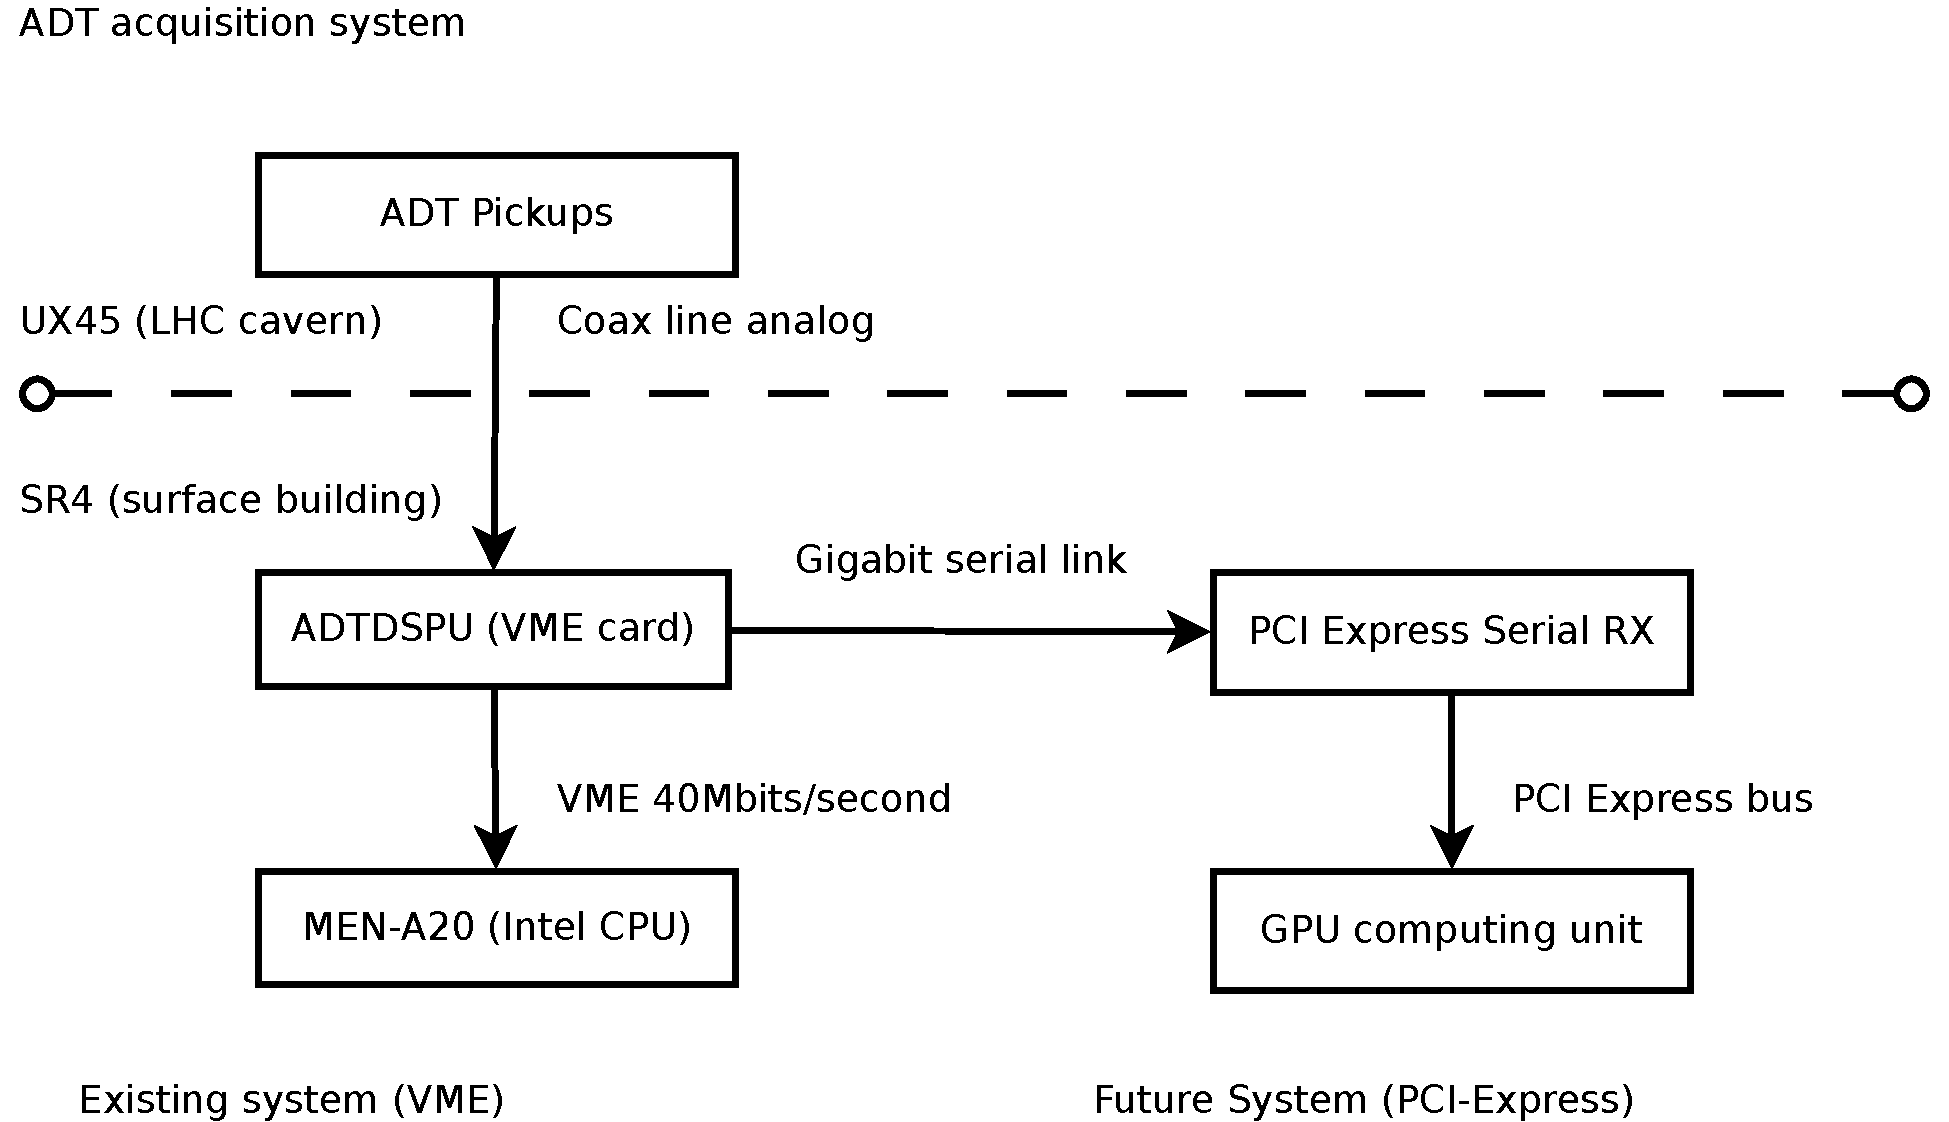
\includegraphics[scale=0.3]{acquisition.pdf}
	\end{figure}

   Per bunch position measurement has to be available to the system for each beam and each plane. This should be provided from the ADTDSPU card and has to be transfered through a serial link to the CPU/GPU crate for computation.

   We need a card in the CPU/GPU crate to de-serialize the data and transfer them to the GPU memory. It may be possible to copy from the acquisition card directly to the GPU memory.

   And finally fast enough GPU to process the data. The number and the type of card should be looked at. The possibility for expansion should be kept as the possibility to implement other algorithms.
   
   \subsection{Timing}

   According to \gls{BI} we have to provide the tune measurement at a rate of between 5 Hz and 10 Hz delay. This mean that the transfer and the computation has to be made in less than 200 ms.

   At a higher frequency because of the acquisition frequency (11 kHz) the precision may be insufficient (Nyquist–Shannon sampling theorem).